\documentclass[french,a4paper]{report}
 
% - taille de la fonte    : 10pt, 11pt, 12pt
% - recto ou recto-verso    : oneside, twoside
 
% Chargement d'extensions
\usepackage[utf8]{inputenc}    
\usepackage{graphicx}
\usepackage{amsmath}
\usepackage{amsfonts}
\usepackage{epsfig}
\usepackage{color}
\usepackage{natbib}
\usepackage{mathrsfs} 
% \usepackage[french]{babel}    
 
% Informations le titre, le(s) auteur(s), la date
\title{X-Light - Analyse des contraintes par diffraction des rayons X}
\author{Guide utilisateur}
\date{\today}

 
 
 
\begin{document}

\sloppy
 
% \maketitle

\begin{titlepage}
\centering
\vfill
{\Huge
X-Light\\
Analyse des contraintes par diffraction des rayons X\\
\Large
\vskip1cm
Guide utilisateur\\
\vskip1cm
\today\\
}    
\vfill
\scalebox{0.2}{
\includegraphics{figures/X-Light.png}}
\vfill
\vfill
\end{titlepage}

\tableofcontents 


\chapter{Introduction}
    
X-Light est un logiciel dédié à l'analyse des contraintes par diffraction des rayons X. Il est développé en langage python et contient un ensemble de fonctionnalités qui peuvent être appelées depuis une interface graphique ou à l'aide de lignes de commande. Le logiciel X-Light permet d'importer des données d'une analyse des contraintes par diffraction réalisée avec des détecteurs ponctuels, linéaires ou plans. Les positions des pics de diffraction contenus dans ces données sont ensuite déterminées, ce qui permet \textit{in fine} d'évaluer l'état de contrainte et les incertitudes associées.

Le présent document est un guide destiné aux utilisateurs du logiciel X-Light. La méthode utilisée pour le calcul des contraintes est détaillée dans la première partie de ce guide. Le fonctionnement d'X-Light est ensuite présenté.

\chapter{Méthode d'analyse des contraintes par diffraction}

Ce premier chapitre a pour objectifs de présenter brièvement la méthode d'analyse des contraintes utilisée au sein d'X-Light ainsi que de préciser les conventions utilisées\footnote{Ce chapitre n'a pas vocation à constituer un document de cours détaillé sur le sujet de l'analyse des contraintes par diffraction. On renvoit le lecteur intéressé vers les ouvrages de référence dédié à ce sujet.}. Il s'agit principalement de fournir à l'utilisateur d'X-Light les informations essentielles sur la méthode utilisée afin qu'il puisse correctement interpréter les résultats obtenus.


\section{Conventions géométriques}

L'analyse des contraintes par diffraction repose sur l'acquisition du signal diffracté par un échantillon lorsqu'il est éclairé par une source de lumière monochromatique. L'acquisition du signal diffracté nécessite d'utiliser un détecteur (ponctuel, linéaire ou surfacique) qui mesure l'intensité du faisceau de lumière diffracté par l'échantillon. Chaque point du détecteur est associé à une direction de mesure (celle du vecteur diffraction), représentée par un vecteur unitaire $\boldsymbol n$. Dans le cas surfacique, un point du détecteur correspond à deux angles appelés $2 \theta$ et $\gamma$. Les valeurs de ces angles dépendent à la fois du pixel considéré ainsi que de la position angulaire $\alpha$ du détecteur sur le cercle goniométrique (voir Figure \ref{fig_bases}). Pour les cas ponctuels ou linéaires, l'angle $\gamma$ est nul tandis que l'angle $2 \theta$ est égal à l'angle $\alpha$.

Les composantes de la direction mesure sont aisément déterminées au sein de la base $\mathcal{E}$ attachée au goniomètre de diffraction à partir des angles $\theta$ et $\gamma$. Comme le montre la Figure \ref{fig_bases}, la base $\mathcal{E}$ est construite à partir de trois vecteurs unitaires mutuellement orthogonaux $(\boldsymbol e_1$, $\boldsymbol e_2$ et $\boldsymbol e_3)$. Spécifiquement, le vecteur $\boldsymbol e_2$ est parallèle au faisceau incident, le vecteur $\boldsymbol e_1$ est orthogonal au cercle goniométrique tandis que le vecteur $\boldsymbol e_3$ est positionné de sorte à former une base orthonormée. Les composantes de la direction mesure $\boldsymbol n$ dans la base $\mathcal{E}$ sont ainsi données par\footnote{Dans un soucis de concision, on utilise les notations $c_\alpha=\cos \alpha$ et $s_\alpha=\sin \alpha$.}:
\begin{equation}
\boldsymbol n =
\begin{bmatrix}
c_\theta s_\gamma \\
-s_\theta  \\
c_\theta c_\gamma
\end{bmatrix}_{\mathcal{E}}
\end{equation}

\begin{figure}
\centering
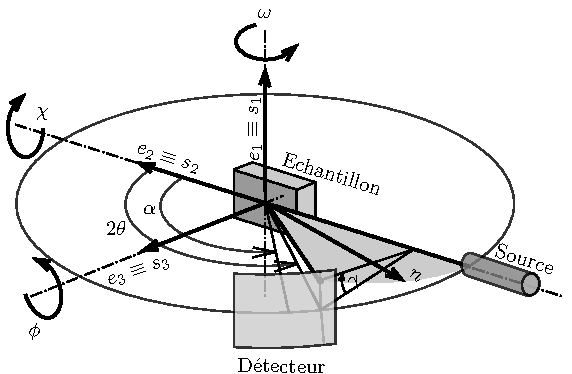
\includegraphics{figures/bases.pdf}
\caption{Représentation schématique d'un échantillon dans un goniomètre de diffraction. Lorsque les angles goniométriques $\chi$, $\phi$ et $\omega$ sont nuls, les vecteurs de la base attachée à l'échantillon coincident avec ceux de la base attachée au goniomètre.}
\label{fig_bases}
\end{figure}

Pour exprimer les résultats de l'analyse des contraintes, il est nécessaire d'associer un système de coordonnées à l'échantillon. Comme le montre la Figure \ref{fig_bases}, la base $\mathcal{S}$ de ce système de coordonnées, formée par trois vecteurs unitaires $\boldsymbol s_1$, $\boldsymbol s_2$ et $\boldsymbol s_3$, est telle que $\boldsymbol s_3$ correspond à la direction normale à la surface externe de l'échantillon tandis que $\boldsymbol s_1$ et $\boldsymbol s_2$ sont contenues dans le plan. L'orientation de la direction de mesure $\boldsymbol n$ vis-à-vis de l'échantillon dépend des angles goniométriques susceptibles d'être contrôlés par l'utilisateur. Pour les diffractomètres équippés d'un berceau d'Euler, les trois angles goniométriques sont généralement notés $\omega$, $\chi$ et $\phi$. Ces angles contrôlent les rotations de l'échantillon autour des axes $\boldsymbol e_1$, $\boldsymbol e_2$ et $\boldsymbol e_3$. Pour l'analyse des contraintes, il est nécessaire d'exprimer les composantes de la direction de mesure $\boldsymbol n$ dans la base attachée à l'échantillon. Cela se fait classiquement à partir des angles $\Phi$ et $\Psi$ qui s'obtiennent à partir de la relation (voir Figure \ref{fig_echantillon}) :
% \begin{equation}
% n'_{i} = R_{ji} ~ n_{j}
% \end{equation}
\begin{equation}
\boldsymbol n =
\begin{bmatrix}
s_\Psi c_\Phi \\
s_\Psi s_\Phi \\
c_\Psi 
\end{bmatrix}_{\mathcal{S}}
=
\begin{bmatrix}
c_\chi c_\phi & c_\omega s_\phi + s_\omega s_\chi c_\phi & s_\omega s_\phi - c_\omega s_\chi c_\phi \\
-c_\chi s_\phi  & c_\omega c_\phi - s_\omega s_\chi s_\phi &   s_\omega c_\phi + c_\omega s_\chi s_\phi\\
s_\chi & -s_\omega  c_\chi & c_\omega  c_\chi  
\end{bmatrix}
\begin{bmatrix}
c_\theta s_\gamma \\
-s_\theta  \\
c_\theta c_\gamma
\end{bmatrix}_{\mathcal{E}}
\end{equation}
La relation précédente est importante en cela qu'elle permet de déterminer pour chaque pixel ($2 \theta$ et $\gamma$) du détecteur la direction de mesure en fonction de l'orientation de l'échantillon représentée par les angles goniométriques ($\omega$, $\chi$ et $\phi$).

\begin{figure}
\centering
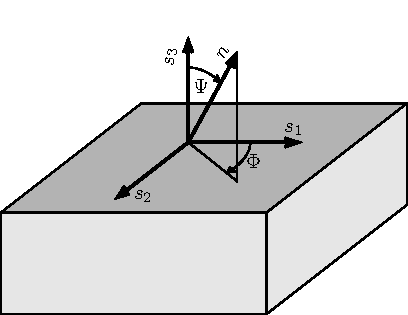
\includegraphics{figures/echantillon.pdf}
\caption{Représentation schématique de la direction de mesure $\boldsymbol n$ dans la base associée à un échantillon. La direction de mesure est orientée à partir des angles $\Psi$ et $\Phi$.}
\label{fig_echantillon}
\end{figure}

\section{Importation et intégration des données}

Lorsque des détecteurs ponctuels ou linéaires sont utilisés, l'analyse des contraintes par les méthodes diffractométriques repose sur la collecte d'un ensemble de profils de diffraction. Chaque profil de diffraction, qui correspond à une direction de mesure, contient un ensemble de points de mesure qui donnent l'intensité $I$ du faisceau diffracté en fonction du double de l'angle d'incidence $2 \theta$. Dans le cas de détecteurs surfaciques, les données d'une analyse de contraintes prennent la forme d'une ou plusieurs images. Chaque image est constituée d'un ensemble de pixels dont le niveau de gris représente l'intensité du faisceau diffracté. Pour exploiter les données obtenues avec un détecteur surfacique, il convient donc d'une part d'associer à chaque pixel $(i,j)$ les valeurs $2 \theta_{i,j}$ et $\gamma_{i,j}$ correspondantes puis, d'autre part, d'intégrer les données pour obtenir des profils de diffraction.

La détermination des angles $2 \theta_{i,j}$ et $\gamma_{i,j}$ pour un pixel exploite les résultats de la calibration du détecteur. La calibration fournit notamment (i) la distance $r$ entre le détecteur et le centre goniométrique, (ii) les coordonnées $(x_c, y_c) $ du centre du détecteur ainsi que (iii) les dimensions $\Delta_x$ et $\Delta_y$ des pixels. A partir des données de calibration, il est possible de déduire les coordonnées $(x_i,y_j)$ d'un pixel $(i,j)$ sur un détecteur bi-dimensionnel à partir des relations :
\begin{align}
&x_{i}= i \times \Delta_x - x_c\\
&y_{j}= j \times \Delta_y-y_c
\end{align}
Aussi, la distance $r$ du détecteur au centre goniométrique et l'angle $\alpha$, qui donne la position du détecteur sur le cercle goniométrique, permettent de déterminer les angles $2 \theta_{i,j}$ et $\gamma_{i,j}$ associés à chaque pixel :
\begin{align}
&2 \theta_{i,j}  = \arccos \left( \frac{x_i \sin \alpha + r \cos \alpha}{r^2+x_i^2+y_j^2} \right) \\
&\gamma_{i,j}  = \text{sign} \left( y_{j}  \right)\arccos \left(  \frac{r \sin \alpha-x_{i} \cos \alpha }{\sqrt{y_{j}^2+(r \sin \alpha-x_{i} \cos \alpha)^2 }} \right)
\end{align}

L'intégration des données nécessite de construire des profils de diffraction, \textit{i.e.} de déterminer l'évolution de l'intensité en fonction de l'angle $2\theta$ pour un angle $\gamma$ fixé. En pratique, il est nécessaire d'introduire des tolérances $\Delta 2 \theta$ et $\Delta \gamma$ pour savoir si le résultat d'un pixel doit être inclus ou non dans un profil de diffraction. Une approche simple (voir Figure \ref{fig_detecteur}) pour l'intégration consiste alors à considérer que l'intensité $I (2 \theta  )$ pour une valeur de $\gamma$ fixée est obtenue en additionnant les intensités $I_{i,j}$ de tous les pixels $(i,j)$ qui vérifient les conditions :
\begin{align}
&2 \theta- \frac{1}{2} \Delta 2 \theta \leq 2 \theta_{i,j}  < 2 \theta+ \frac{1}{2} \Delta 2 \theta \\
&\gamma- \frac{1}{2} \Delta \gamma \leq \gamma_{i,j}  < \gamma+ \frac{1}{2} \Delta \gamma 
\end{align}
L'importation d'un ensemble d'images obtenues avec un détecteur surfacique permet donc, après intégration, de retrouver une situation semblable à celle des détecteurs ponctuels ou linéaires. On dispose en effet de différents profils de diffraction $I (2 \theta  )$ à chacun desquels est associé un quadruplet d'angles $(\gamma,\omega,\chi,\phi)$.

\begin{figure}
\centering
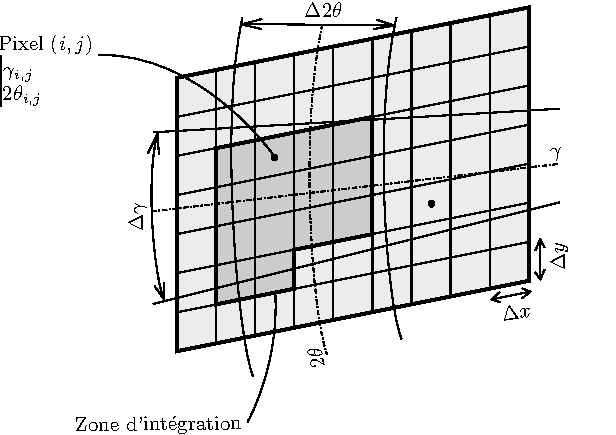
\includegraphics{figures/detecteur.pdf}
\caption{Procédure d'intégration pour la construction d'un profil de diffraction à partir d'une image bi-dimensionnelle.}
\label{fig_detecteur}
\end{figure}

\section{Correction des profils de diffraction}

Avant d'exploiter les profils de diffraction, il est parfois nécessaire d'appliquer un ensemble de corrections à l'intensité mesurée. L'effet de ces corrections est généralement regroupé sous la forme du produit $PLA$ qui intègre les corrections de polarisation, de Lorentz et d'absorption. La correction de polarisation $P$ dépend des angles $2 \theta$ et $\gamma$ au travers de la relation :
\begin{equation}
P = \frac{\left( 1+\cos^2  2 \theta  \cos^2  2 \theta_m  \right) \cos^2 \gamma +\left( \cos^2  2 \theta  + \cos^2  2 \theta_m  \right) \sin^2 \gamma }{1+\cos^2  2 \theta_m }
\end{equation}
où $\theta_m$ est l'angle de Bragg associé à l'éventuel monochromateur (l'angle $\theta_m$ est nul en l'absence de monochromateur).

Pour les diffractomètres conventionnels, le facteur de Lorentz $L$ s'exprime à partir de l'angle d'incidence $\theta$ comme suit :
\begin{equation}
L = \frac{1}{ \sin^2  \theta  }
\end{equation}

Enfin, pour un échantillon dont l'épaisseur est très grande par rapport à la profondeur de pénétration du rayonnement, le facteur $A$, qui permet de tenir compte des éventuels phénomènes d'absorption, est donné par :
\begin{equation}
A = \frac{\cos \beta }{  \left(\cos \beta + \cos \zeta \right)} %\cos \zeta
\end{equation}
avec :
\begin{align}
&\cos \beta = \sin \omega \cos \chi\\
&\cos \zeta = \sin 2 \theta \sin \gamma \sin \chi + \sin 2 \theta \cos \gamma \cos \omega \cos \chi -\cos 2 \theta \sin \omega \cos \chi
\end{align}
Les angles $\beta$ et $\zeta$ qui interviennent dans la relation précédente correspondent aux angles qui séparent la normale à l'échantillon $\boldsymbol s_3$ respectivement du faisceau incident et du faisceau diffracté. Ces angles permettent de calculer la profondeur de pénétration $\tau$ à partir de la relation :
\begin{equation}
\tau = \frac{\cos \beta \cos \alpha}{ \mu \left(\cos \beta + \cos \zeta \right)} %\cos \zeta
\end{equation}
où $\mu$ est le coefficient d'absorption linéaire.

L'intensité corrigée $i$ se déduit alors de l'intensité mésurée $I$ à partir de la relation :
\begin{equation}
i = \frac{I}{PLA \times t}
\end{equation}
où $t$ représente le temps de comptage. La normalisation par le temps de comptage fournit une intensité dont l'unité correspond à un nombre de coups par unité de temps. Bien que cela ne soit pas absolument nécessaire pour l'exploitation des signaux de diffraction, la normalisation par le temps de comptage permet la comparaison directe entre des profils de diffraction obtenus pour des temps de comptage différents. Aussi, pour l'évaluation des incertitudes statistiques, il est nécessaire de connaître l'incertitude $\delta i$ associé à la mesure d'intensité $i$. En supposant que le comptage des photons est assimilable à un processus de Poisson, l'incertitude $\delta i$ est donnée par :
\begin{equation}
\delta i = \sqrt{\frac{i}{ PLA \times t}}
\end{equation}

De la même manière, afin de s'affranchir de la dépendance à la longueur d'onde, il est commode de représenter l'intensité en fonction de la norme $q$ du vecteur diffraction qui s'exprime en fonction de l'angle d'incidence $\theta$ à partir de la relation : 
\begin{equation}
q = \frac{4 \pi \sin \theta}{\lambda}
\end{equation}
où $\lambda$ est la longueur d'onde du rayonnement utilisé\footnote{Lorsque le rayonnement utilisé contient les contributions des raies $K_{\alpha 1}$ et $K_{\alpha 2}$ (de longueur d'onde respective $\lambda_{\alpha 1}$ et $\lambda_{\alpha 2}$), la longueur d'onde $\lambda$ est donnée par la relation $\lambda = (\lambda_{\alpha 1} + r \lambda_{\alpha 2})/(1+r)$, où $r$ est le rapport d'intensité entre ces deux contributions.}.

L'étape de correction permet ainsi d'obtenir un ensemble de profils de diffraction qui peuvent ensuite être analysés pour estimer les positions des pics de diffraction.

\section{Localisation des pics de diffraction}

Afin d'évaluer l'état de contrainte, il est nécessaire d'estimer la position des pics de diffraction qui composent un profil de diffraction. Une méthode possible consiste à ajuster une fonction $i(q )$ pour représenter au mieux un profil de diffraction. Pour ce faire, il convient d'identifier un ensemble de paramètres à partir des données expérimentales. En règle générale, il est possible de classer les paramètres en deux catégories. Spécifiquement, certains paramètres servent à décrire les $p$ pics de diffraction qui composent un profil tandis que les autres permettent de représenter le bruit de fond. Il est donc possible de décomposer la fonction $i$ de manière additive comme suit :
\begin{equation}
 i \left(q \right) = b \left(q  \right) + \sum_{hkl} f_{hkl} \left(q  \right)
\end{equation}
où $b$ représente la contribution du bruit de fond tandis que $f_{hkl}$ représente la contribution de la réflection $\{ hkl \}$ au signal diffracté.

Pour l'analyse des contraintes, le bruit de fond est classiquement représenté par un polynôme d'ordre $n$ qui fait intervenir $n+1$ paramètres :
\begin{equation}
 b \left(q \right) = b_0 + b_1 q + b_2 q^2 + ...+ b_n q^n
\end{equation}
où les $b_i$ (avec $i=0, ... n$) sont les paramètres du bruit de fond. Aussi, pour représenter les pics de diffraction, différentes fonctions $f_{hkl}$ sont communément utilisées (voir Tableau \ref{tab_fonction}). Si le nombre de paramètres $m$ utilisé par ces fonctions est variable selon la forme retenue, elles utilisent \textit{a minima} un paramètre d'intensité $i_{hkl}$, un paramètre de position $q_{hkl}$ et un paramètre de largeur $w_{hkl}$. A ces paramètres peuvent s'ajouter d'éventuels paramètres de forme et d'asymétrie. Aussi, pour précisémment localiser un pic de diffraction, il est parfois nécessaire de tenir compte du doublet $K_{\alpha 1} / K_{\alpha 2}$. Pour ce faire, la fonction $f_{hkl} $ associée à la réflection $\{ hkl \}$ est décomposée en deux contributions :
\begin{equation}
f_{hkl} \left(q \right) = f^1_{hkl} \left(q \right) + r f^2_{hkl} \left(q \right)
\end{equation}
% \begin{equation}
% f_{hkl} \left(q , a_0, a_1, a_2...\right) = f^1 \left(q , a_0, a_1, a_2...\right) + r f^2_{hkl} \left(q, a_0, a_1 \times \lambda_{\alpha 2} / \lambda_{\alpha 1}, a_2... \right)
% \end{equation}
où $r$ désigne le rapport d'intensité entre les contributions $K_{\alpha 1}$ et $K_{\alpha 2}$. Les fonctions $f^1_{hkl}$ et $f^2_{hkl}$ sont identiques, elles utilisent les mêmes paramètres à ceci près que la position de la contribution $K_{\alpha 2}$ est décalée par rapport à celle de  $K_{\alpha 1}$\footnote{Si la position de la contribution $f^1_{hkl}$ est $a_1^{hkl}$, celle de la contribution $f^2_{hkl}$ correspond à $a_1^{hkl}\times \lambda_{\alpha 2} / \lambda_{\alpha 1}$.}. L'ampleur de ce décalage dépend du rapport entre les longueurs d'onde $\lambda_{\alpha 1}$ et  $\lambda_{\alpha 2}$.

\begin{table}
\centering
\begin{tabular}{ll}
\hline
Fonction & Définition \\
\hline
& \\
Gauss & \\
\quad symétrique & $g_s (x)=i \exp \left( - \ln 2 \left( \frac{x-q}{w}\right)^2\right)$ \\
& \\
\quad asymétrique & $g_a(x)=i \exp \left( - \ln 2 \left( \frac{x-q}{w}\right)^2\right)$ si $x \geq q$ \\
& $g_a(x)=i \exp \left( - \ln 2 \left( \frac{x-q}{w'}\right)^2\right)$ si $x < q$ \\
& \\
\hline
& \\
Lorentz & \\
\quad symétrique & $l_s(x)= i \left(   1+ \left(\frac{x-q}{w}\right)^2\right)^{-1}$ \\
& \\
\quad asymétrique & $l_a(x)= i \left(   1+ \left(\frac{x-q}{w}\right)^2\right)^{-1}$ si $x \geq q$ \\
& $l_a(x)= i \left(  1+ \left(\frac{x-q}{w'}\right)^2\right)^{-1}$ si $x < q$ \\
& \\
\hline
& \\
Pseudo-Voigt & \\
\quad symétrique & $v_s(x)=(1 -s) g_s+ s l_s$ \\
& \\
\quad asymétrique & $v_a(x)=(1 -s) g_a+ s l_a$  \\
& \\
\hline
& \\
Pearson VII & \\
\quad symétrique & $p_s(x)=i \left(   1+ \left(\frac{x-q}{w}\right)^2 \left( 2^{1/s}-1\right)\right)^{-s}$  \\
& \\
\quad asymétrique & $p_a (x) =i \left(   1+ \left(\frac{x-q}{w}\right)^2 \left( 2^{1/s}-1\right)\right)^{-s}$ si $x \geq q$  \\
 & $p_a(x)=i \left(   1+ \left(\frac{x-q}{w'}\right)^2 \left( 2^{1/s}-1\right)\right)^{-s}$ si $x <q$  \\
 & \\
\hline
\end{tabular}
\caption{Liste des fonctions communément utilisées pour décrire un pic de diffraction. La variable dont dépend la fonction est notée $x$. Les paramètres $i$, $q$, $w$, $w'$ et $s$ contrôlent respectivement l'intensité, la position, les demi-largeurs (droite et gauche) et la forme d'un pic de diffraction.}
\label{tab_fonction}
\end{table}

L'étape de localisation doit \textit{in fine} conduire à un ensemble de paramètres qui décrivent au mieux un profil de diffraction. Le nombre total de paramètres correspond à l'addition du nombre de paramètres nécessaire au bruit de fond (\textit{i.e.} $n+1$) et du nombre de paramètres nécessaire à la description de l'ensemble des pics de diffraction (\textit{i.e.} $m \times p$). Ces paramètres sont obtenus par une procédure d'optimisation qui cherche à minimiser l'écart quadratique entre les valeurs d'intensité obtenues expérimentalement et celles calculées à partir de la fonction de modélisation choisie. Outre les valeurs optimales des paramètres, la procédure d'optimisation fournit également les incertitudes statistiques associées.

\section{Détermination des contraintes}

La détermination des contraintes au sein d'un matériau polycristallin repose sur le calcul des déformations élastiques résultant de l'application d'un état de contrainte. La déformation réticulaire $\varepsilon_{hkl}$ d'une famille de plans $\{hkl\}$ du réseau cristallin selon une direction de mesure $\boldsymbol n$ est classiquement calculée à partir de la distance interréticulaire $d_{hkl}$ en utilisant la relation :
\begin{equation}
\varepsilon_{hkl} (\boldsymbol n) = \frac{d_{hkl}(\boldsymbol n)}{d^0_{hkl}}-1
\end{equation}
où $d^0_{hkl}$ représente la distance interréticulaire séparant les plans $\{hkl\}$ en l'absence de contrainte. L'étape de localisation décrite précédemment ne fournit pas directement les distances interréticulaires $d_{hkl}$ mais les positions $q_{hkl}$ (ainsi que les incertitudes associées) des pics qui composent les profils de diffraction d'une analyse. Ces deux grandeurs sont liées l'une à l'autre par la relation :
\begin{equation}
q_{hkl} (\boldsymbol n) = \frac{2 \pi}{d_{hkl}(\boldsymbol n)}
\end{equation}
La relation précédente permet d'exprimer la déformation comme suit :
\begin{equation}
\varepsilon_{hkl} (\boldsymbol n) = \frac{q^0_{hkl}}{q_{hkl}(\boldsymbol n)}-1
\label{eq_strain_q}
\end{equation}
où $q^0_{hkl}$ représente la position du pic de diffraction $\{hkl\}$ en l'absence de contrainte.

Il est possible d'exprimer les déformations réticulaires en fonction du tenseur des contraintes $\boldsymbol \sigma$ à partir du tenseur $\boldsymbol F_{hkl}$. Ce dernier caractérise la souplesse d'un matériau selon une direction unitaire $\boldsymbol n$ pour une famille de plans réticulaires $\{hkl\}$ particulière de sorte que :
\begin{equation}
\varepsilon_{hkl} (\boldsymbol n) = \boldsymbol F_{hkl} (\boldsymbol n) : \boldsymbol \sigma
\label{eq_strain_stress}
\end{equation}
Le tenseur de souplesse $\boldsymbol F_{hkl}$ est exprimé à partir du module de Young $E_{hkl}$ et du coefficient de Poisson $\nu_{hkl}$ en utilisant la relation\footnote{Les propriétés de souplesse peuvent également être déterminées à partir des constantes d'élasticité radio-cristallographiques en utilisant les relations $1/2 s_{2,hkl}= (1+\nu_{hkl})/E_{hkl}$ et $ s_{1,hkl}= -\nu_{hkl}/E_{hkl}$.} :
\begin{equation}
\boldsymbol F_{hkl} (\boldsymbol n) = \frac{1+\nu_{hkl}}{E_{hkl}} \boldsymbol n \otimes \boldsymbol n - \frac{\nu_{hkl}}{E_{hkl}} \boldsymbol I 
\end{equation}

Le système linéaire qui permet de déterminer l'état de contrainte $\boldsymbol \sigma$ s'obtient en combinant les relations \eqref{eq_strain_q} et \eqref{eq_strain_stress}, ce qui conduit à :
\begin{equation}
q^0_{hkl}-q_{hkl}(\boldsymbol n) =q_{hkl}(\boldsymbol n) \boldsymbol F_{hkl} (\boldsymbol n) : \boldsymbol \sigma
\end{equation}
Différentes hypothèses peuvent être adoptées pour la résolution de ce système linéaire. D'abord, il est possible de supposer que le tenseur des contraintes prend une forme spécifique, en particulier que certaines composantes sont nulles. Les états de contrainte couramment utilisés sont précisés dans le Tableau \ref{tab_contrainte}. 

\begin{table}
\centering
\begin{tabular}{lll}
\hline
\hline
\\[-1em]
Etat de contrainte & Surface & Composantes non-nulles\\
\hline
\\[-1em]
Uniaxial selon $\boldsymbol s_1$ & Libre & $\sigma_{11}$ \\
\hline
\\[-1em]
Uniaxial selon $\boldsymbol s_2$ & Libre & $\sigma_{22}$ \\
\hline
\\[-1em]
Biaxial selon $\boldsymbol s_1$ et $\boldsymbol s_2$ & Libre & $\sigma_{11}$, $\sigma_{12}$ et $\sigma_{22}$ \\
\hline
\\[-1em]
Triaxial & Libre & $\sigma_{11}$, $\sigma_{12}$, $\sigma_{22}$, $\sigma_{23}$ et $\sigma_{31}$\\
\\[-1em]
 & Non-libre & $\sigma_{11}$, $\sigma_{12}$, $\sigma_{22}$, $\sigma_{23}$, $\sigma_{33}$ et $\sigma_{31}$\\
\hline
\hline
\end{tabular}
\caption{Etats de contraintes particuliers utilisables pour l'analyse des contraintes. La présence d'une surface libre suppose que la contrainte normale $\sigma_{33}$ est nulle.}
\label{tab_contrainte}
\end{table}

Aussi, dans de nombreuses situations pratiques, les positions de référence $q^0_{hkl}$ des différents plans réticulaires qui contribuent aux profils de diffraction ne sont pas connues avec précision. Ces positions de référence constituent alors des inconnues du problème de l'analyse des contraintes. Elles doivent donc être déterminées à partir des positions $q_{hkl}$ au même titre que l'état de contrainte. Pour ce faire, il convient de supposer que la surface externe de l'échantillon est libre et que la contrainte normale correspondante est nulle (\textit{i.e.} $\sigma_{33}=0$). Il existe néanmoins de rares cas où les positions de référence sont connues, elles sont alors considérées comme des données du problème au même titre que les positions $q_{hkl}$.

Quelles que soient les hypothèses retenues, la détermination des contraintes prend la forme d'un problème linéaire dont la résolution conduit à l'état de contrainte $\boldsymbol \sigma$, ainsi qu'à l'incertitude statistique associée $\delta \boldsymbol \sigma$, à partir des positions $q_{hkl}$ des pics de diffraction et des incertitudes statistiques associées $\delta q_{hkl}$.


\chapter{Interface utilisateur}

L'interface graphique d'X-Light est décrite dans ce second chapitre. Les paquets nécessaires à l'installation sont d'abord listés. Les fonctionnalités contenues dans les différents onglets qui composent l'interface sont ensuite détaillées. Le format des fichiers qui constituent la base de données d'X-Light est exposé dans la dernière partie de ce chapitre.


\section{Installation et exécution}

Le logiciel X-light est développé en langage Python. Pour fonctionner correctement, X-light nécessite la version 3.7 de Python ou une version ultérieure. Aussi, l'installation préalable des paquets suivants est requise~:
\begin{itemize}
\item{numpy (1.19 ou supérieure),}
\item{matplotlib (3.5 ou supérieure),}
\item{PySide6 (6.1 ou supérieure),}
\item{scipy (1.6 ou supérieure),}
\item{numba (0.54 ou supérieure).}
\end{itemize}
Le lancement de l'interface graphique s'effectue depuis le répertoire \texttt{X-light} à l'aide de la commande~:\\
\texttt{Python -m xlight}

\section{Utilisation}

L'interface graphique d'X-Light (voir Figure \ref{fig_import}) prend la forme de quatre onglets (\texttt{Import}, \texttt{Inspect}, \texttt{Localize} et \texttt{Evaluate}). Chacun de ces onglets est associé à une des étapes de l'analyse des contraintes. En particulier, le premier onglet permet l'importation de données. Le second onglet permet la visualisation des profils de diffraction contenus dans les fichier de données. Le troisième onglet contient tous les aspects liés à la localisation des pics de diffraction. L'évaluation des contraintes en tant que telle est réalisée à partir du dernier onglet.


\subsection{Importation}

L'onglet d'importation contient deux commandes (\texttt{Import data} et \texttt{Clear data}). La lecture des fichiers de données est réalisée à partir de la commande \texttt{Import data}. Les formats des fichiers acceptés par X-Light sont \textit{nja}, \textit{uxd} et \textit{gfrm}. Il est possible de réaliser une analyse de contraintes à partir des données issues de différents fichiers. Ces fichiers peuvent être importés en une seule ou en plusieurs fois à partir de la commande \texttt{Import data}. Lorsque les fichiers correspondent à des images (\textit{gfrm}), l'importation nécessite de préciser les tailles $\Delta 2 \theta$ et $\Delta \gamma$ de la fenêtre d'intégration. Aussi, il convient de préciser les longueurs d'onde correspondant à l'anode utilisée pour générer le rayonnement. Pour ce faire, X-Light utilise une base de données qui contient les caractéristiques des anodes courantes (voir \ref{sec_fichieranode}). Pour les données obtenues à partir d'un détecteur 2D, la base de données d'X-Light doit également inclure le détecteur correspondant et les données de calibration associées (voir \ref{sec_fichierdetecteur}).

La commande \texttt{Clear data} efface l'ensemble des données, ainsi que les résultats associés. Cette commande permet de réaliser différentes analyses de contrainte sans que cela nécessite de relancer X-Light.


\begin{figure}[h!]
\centering
\scalebox{0.18}{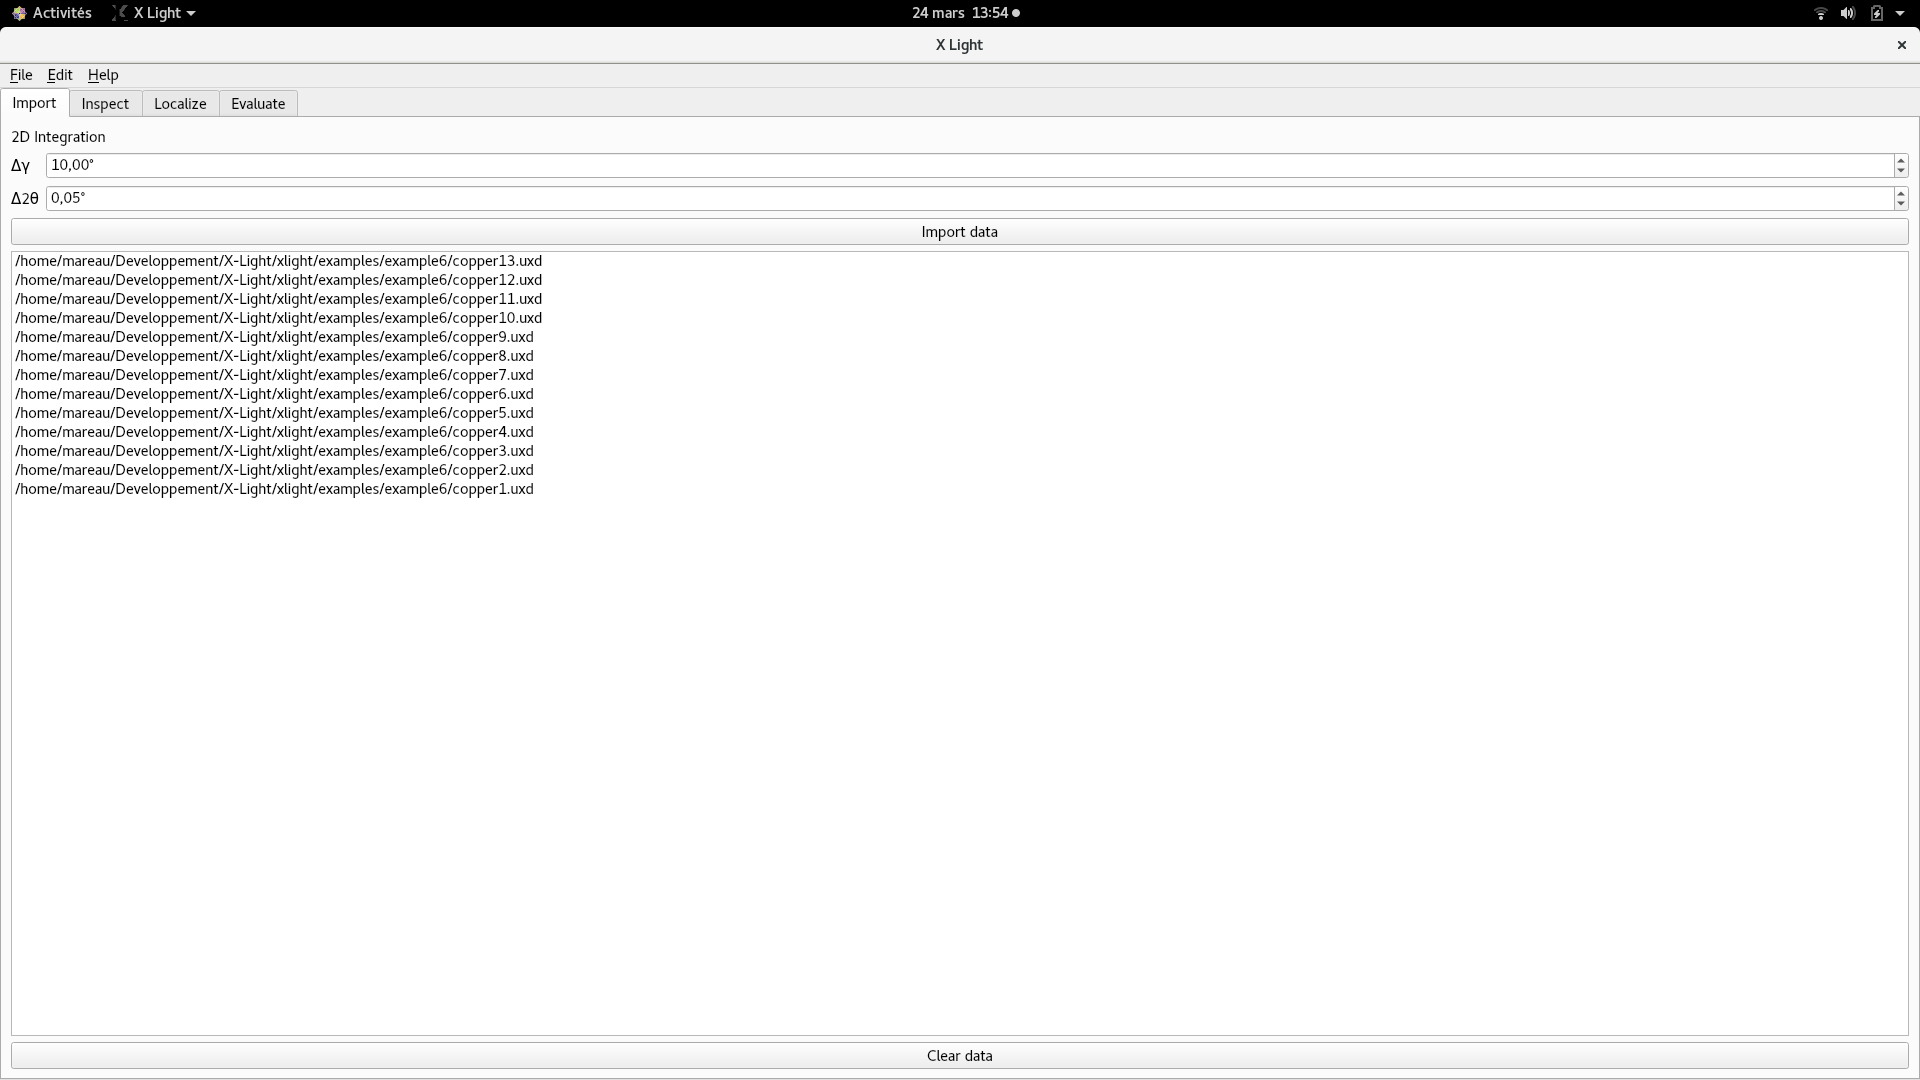
\includegraphics{figures/import.png}}
\caption{Vue de l'onglet importation de l'interface d'X-Light.}
\label{fig_import}
\end{figure}

\subsection{Inspection}

\label{sec_visualisation}

Les profils de diffraction obtenus après importation sont visibles sous la forme de diagrammes représentant l'intensité $I$ en fonction de l'angle $2\theta$ depuis l'onglet inspection (voir Figure \ref{fig_inspect}). Les données associées à chaque profil (longueur d'onde, angles goniométriques) sont présentées à droite du diagramme, qui inclut également des fonctionnalités de zoom et de translation. Il est possible de basculer entre les différents profils à partir des commandes $<<$, $<$, $>$ et $>>$ situées au-dessus du diagramme $I-2\theta$. Il est important de noter que les graphiques sont complétés après l'étape de localisation par les profils modélisés, qui viennent ainsi s'ajouter aux profils expérimentaux. L'option \texttt{Enabled/Disabled} permet d'activer/désactiver un profil de diffraction. Les données obtenues à partir des profils désactivés ne sont pas considérées lors de l'évaluation des contraintes.

\begin{figure}[h!]
\centering
\scalebox{0.18}{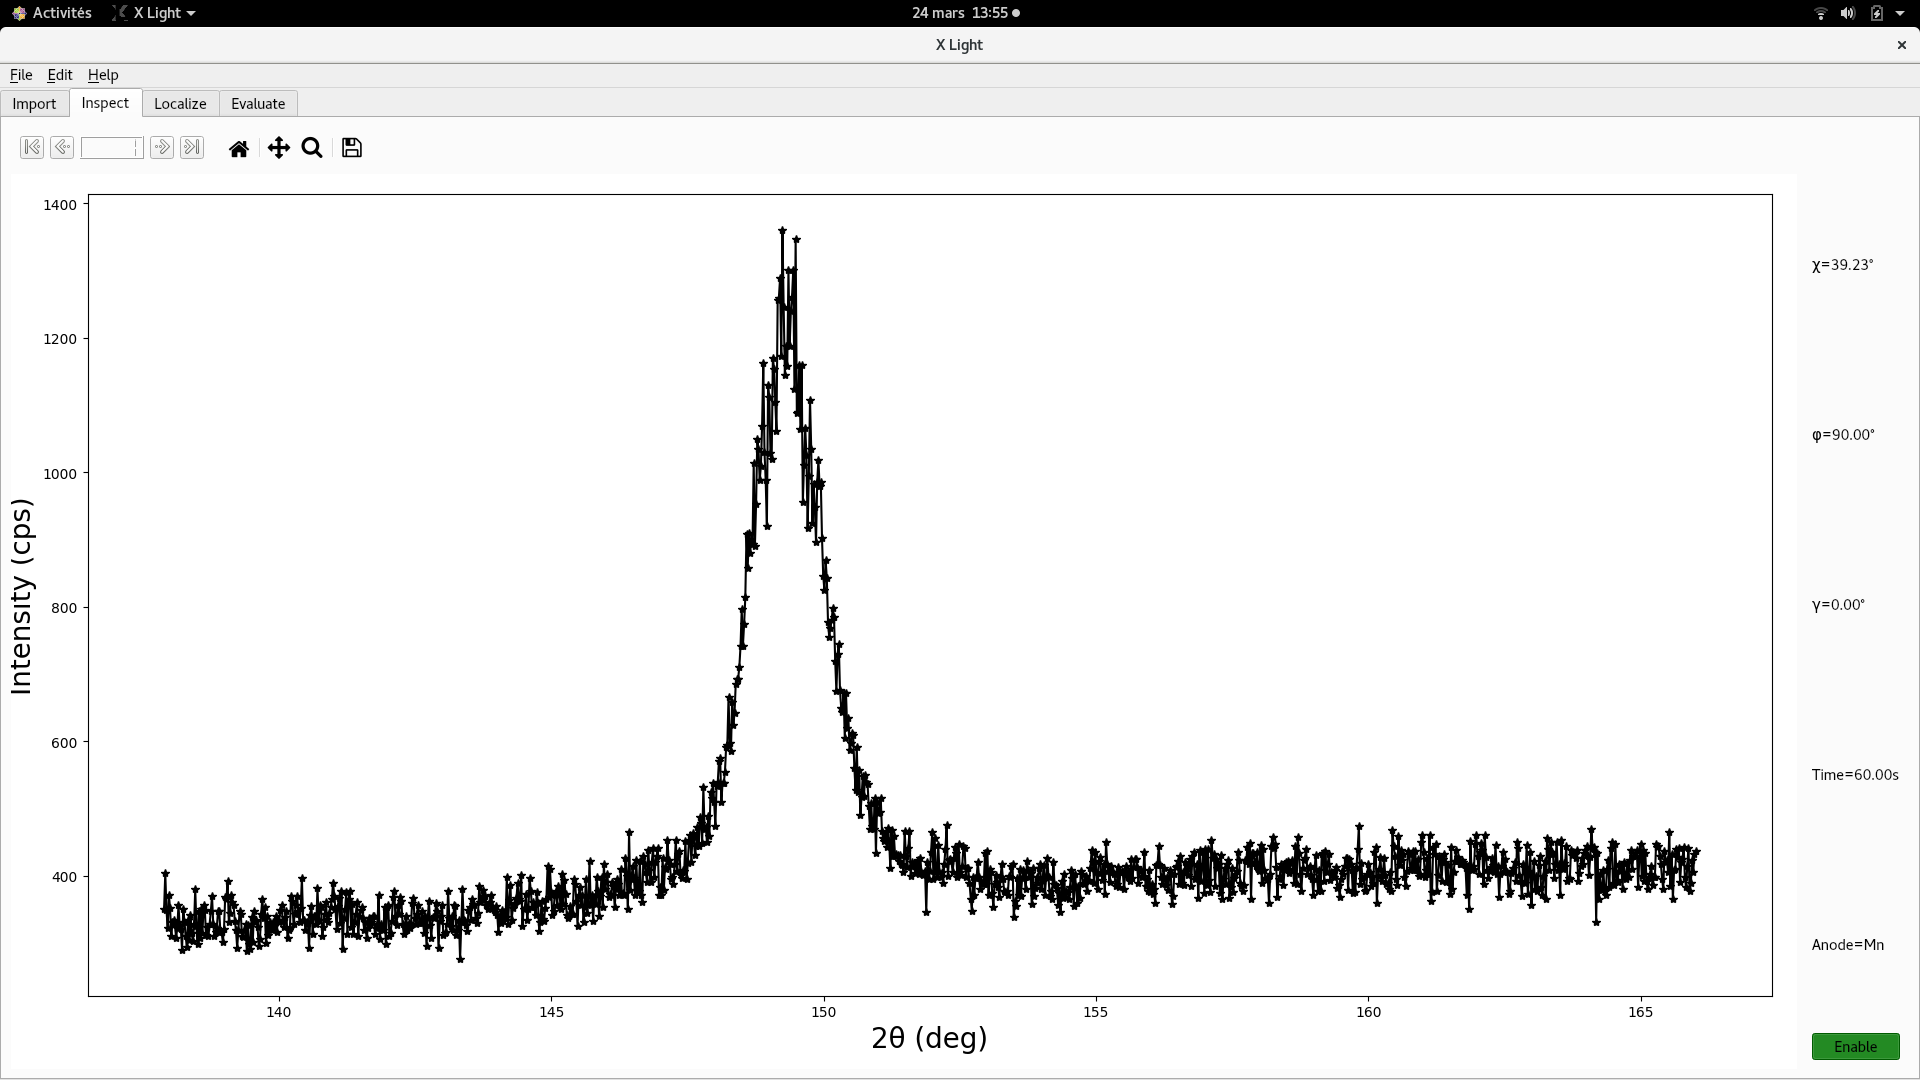
\includegraphics{figures/inspect.png}}
\caption{Vue de l'onglet inspection de l'interface d'X-Light.}
\label{fig_inspect}
\end{figure}

\subsection{Localisation}

Les options disponibles pour la localisation des pics de diffraction sont contenues dans l'onglet du même nom (voir Figure \ref{fig_localize}). L'utilisateur peut choisir d'appliquer certaines corrections (\texttt{Lorentz}, \texttt{Polarisation}, \texttt{Absorption}) aux profils de diffraction en amont de l'étape de localisation. Par défaut, aucune correction n'est appliquée aux profils de diffraction.

Pour la localisation des pics de diffraction, X-light utilise les fichiers matériau disponibles dans la base de données (voir \ref{sec_fichiermateriau}). Spécifiquement, à partir des paramètres de maille de la phase métallurgique (matériau) choisie, X-Light détermine les positions théoriques des différentes familles de plans réticulaires $\{hkl\}$. Pour chaque profil, X-Light est alors en mesure d'identifier les familles susceptibles de contribuer au signal diffracté.


\begin{figure}[bh!]
\centering
\scalebox{0.18}{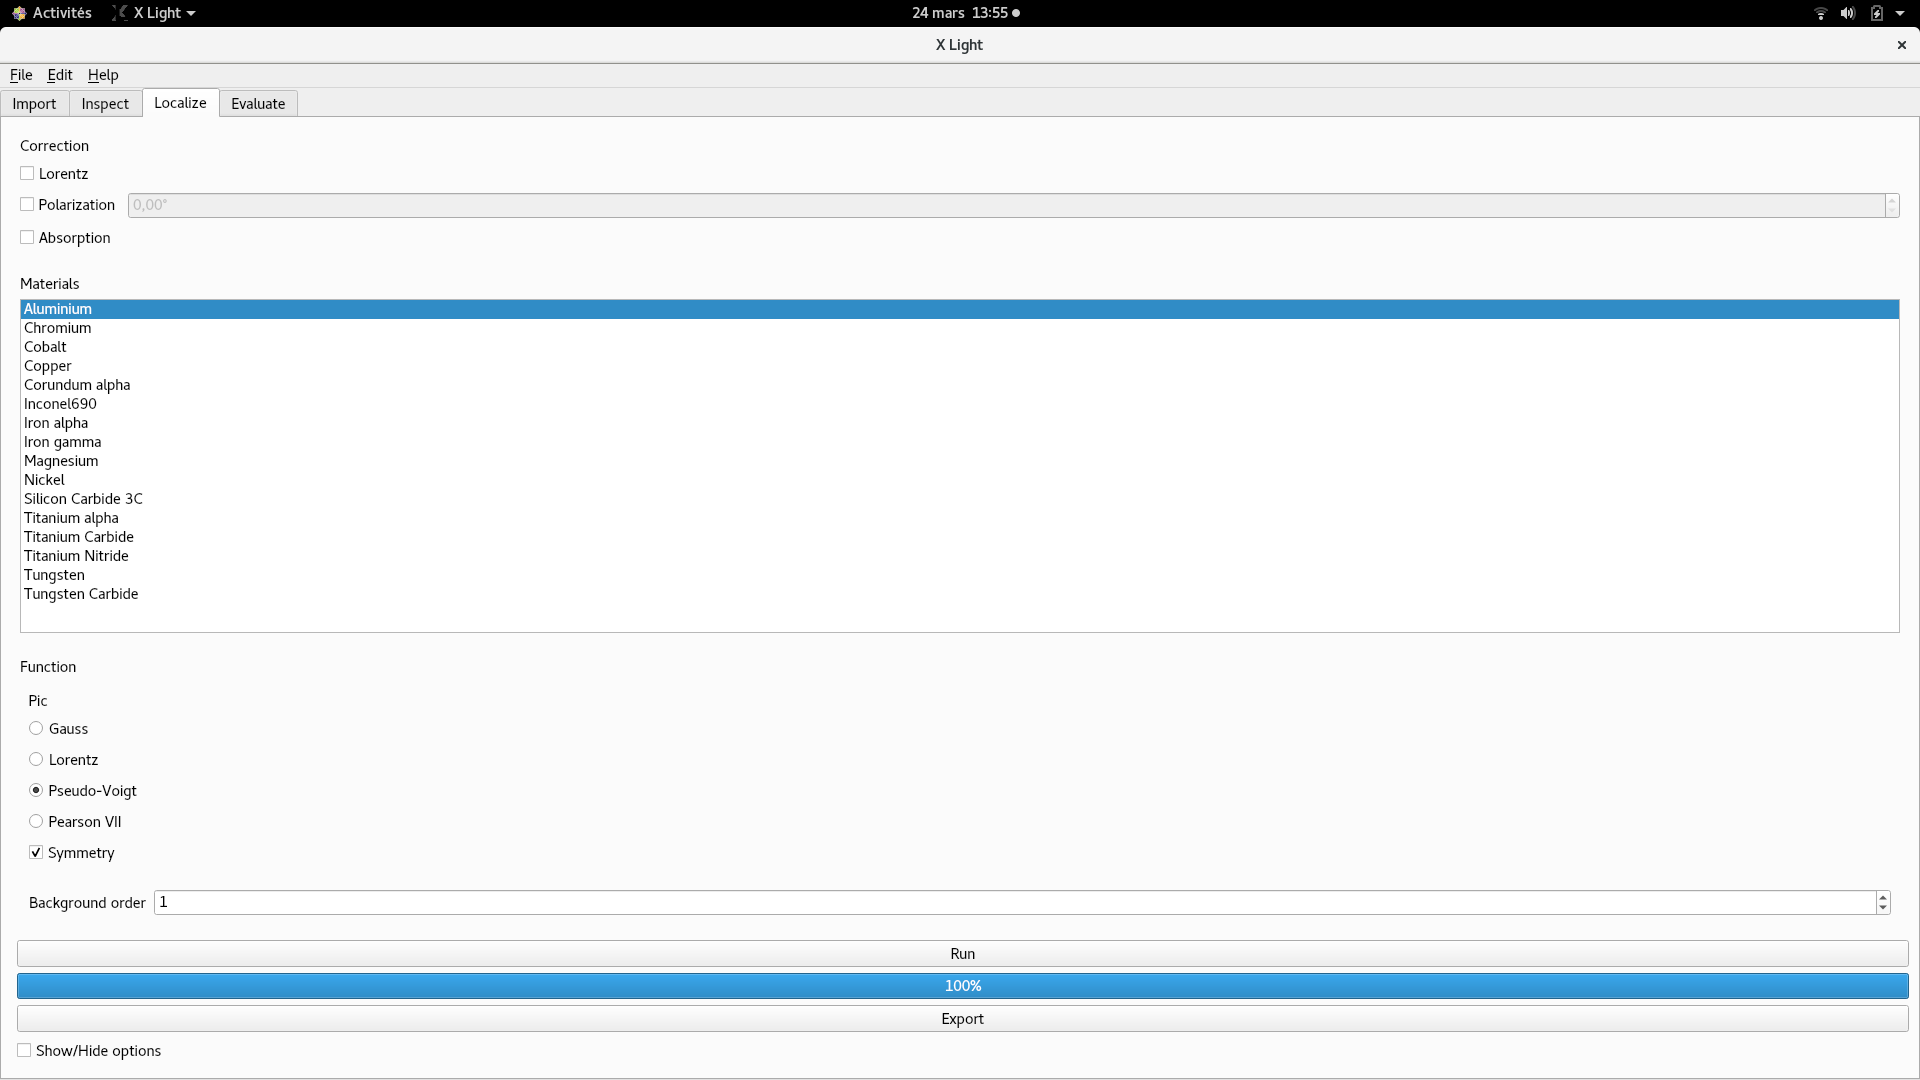
\includegraphics{figures/localize.png}}
\caption{Vue de l'onglet localisation de l'interface d'X-Light.}
\label{fig_localize}
\end{figure}

La localisation précise des pics de diffraction nécessite d'indiquer la fonction de modélisation des pics (\texttt{Gauss}, \texttt{Lorentz}, \texttt{Pseudo-Voigt} ou \texttt{Pearson VII}) ainsi que l'ordre du polynôme utilisé (\texttt{Background order}) pour représenter le bruit de fond. Une option permet également d'indiquer si la fonction de modélisation des pics de diffraction est symétrique ou non. Il convient de préciser que seul un type de fonction peut être utilisé pour l'ensemble des données d'une analyse.

L'application des corrections puis la localisation ne sont effectuées par X-Light que lorsque la commande \texttt{Run} est lancée. X-Light utilise une procédure de localisation globale au sens où les paramètres du bruit de fond et des pics de diffraction sont optimisés simultanément. Après l'étape de localisation, il est possible de comparer les données expérimentales à la modélisation dans l'onglet de visualisation (voir \ref{sec_visualisation}). Les résultats de la localisation vers un fichier texte peuvent également être exportés vers un fichier texte à partir de la commande \texttt{Export}.

X-light utilise une procédure d'optimisation pour déterminer tous les paramètres (pics et bruit de fond) d'un profil de diffraction. Cette procédure d'optimisation requiert des estimations initiales de l'ensemble des paramètres. L'estimation initiale des paramètres du bruit de fond repose sur une méthode itérative qui fait appel à une tolérance permettant de définir quels sont les points utilisés pour réaliser cette estimation. La valeur de cette tolérance est contrôlée à partir des options avancées (\texttt{Show/Hide options} puis \texttt{Background tolerance}). X-light réalise ainsi une première estimation du bruit de fond à partir de l'ensemble des données contenues dans un profil. Il exclue ensuite tous les points dont l'intensité est, à la tolérance relative près, supérieure au bruit de fond. Il réalise ensuite une seconde estimation des paramètres de bruit de fond avec un nombre réduit de points expérimentaux. Les points d'intensité trop élevée sont à nouveau exclus. Cette procédure itérative est répétée jusqu'à ce que le nombre de points utilisés pour évaluer les paramètres de bruit de fond n'évolue plus. X-Light utilise ensuite les données disponibles au voisinage de la position attendue de chaque pic pour réaliser une estimation de la position, de l'intensité et de la largeur des différents pics de diffraction dans chacun des profils de diffraction. Cette première estimation est obtenue à partir d'une méthode du barycentre, appliquée aux données contenues dans une fenêtre centrée sur la position attendue. La taille relative de cette fenêtre est contrôlée à partir des options avancées \texttt{Show/Hide options} puis \texttt{Peak tolerance}. Ainsi, si on appelle $\theta$ cette tolérance, X-light utilise les données dont la position est comprise entre $(1-\theta)\times q^0_{hkl}$ et $(1+\theta)\times q^0_{hkl}$ pour déterminer approximativement la position, l'intensité et la largeur du pic de diffraction associée à la famille de plans réticulaires $\{hkl\}$.

\subsection{Evaluation}

L'évaluation de l'état de contrainte est possible dès lors que la localisation des pics de diffraction a été effectuée. L'onglet d'évaluation (voir Figure \ref{fig_evaluate}) permet de formuler \textit{a priori} une hypothèse sur l'état de contrainte. Les états de contrainte possibles sont ceux présentés dans le Tableau \ref{tab_contrainte}. La commande \texttt{Run} permet d'effectuer le calcul de l'état de contrainte et des incertitudes associées. Outre la présentation matricielle des résultats, l'onglet d'évaluation donne également les contraintes équivalentes de von Mises, Tresca ainsi que la pression hydrostatique. Si une autre hypothèse quant à la forme de l'état de contrainte est adoptée, il convient de relancer la commande \texttt{Run} pour mettre à jour les résultats.

\begin{figure}[bh!]
\centering
\scalebox{0.18}{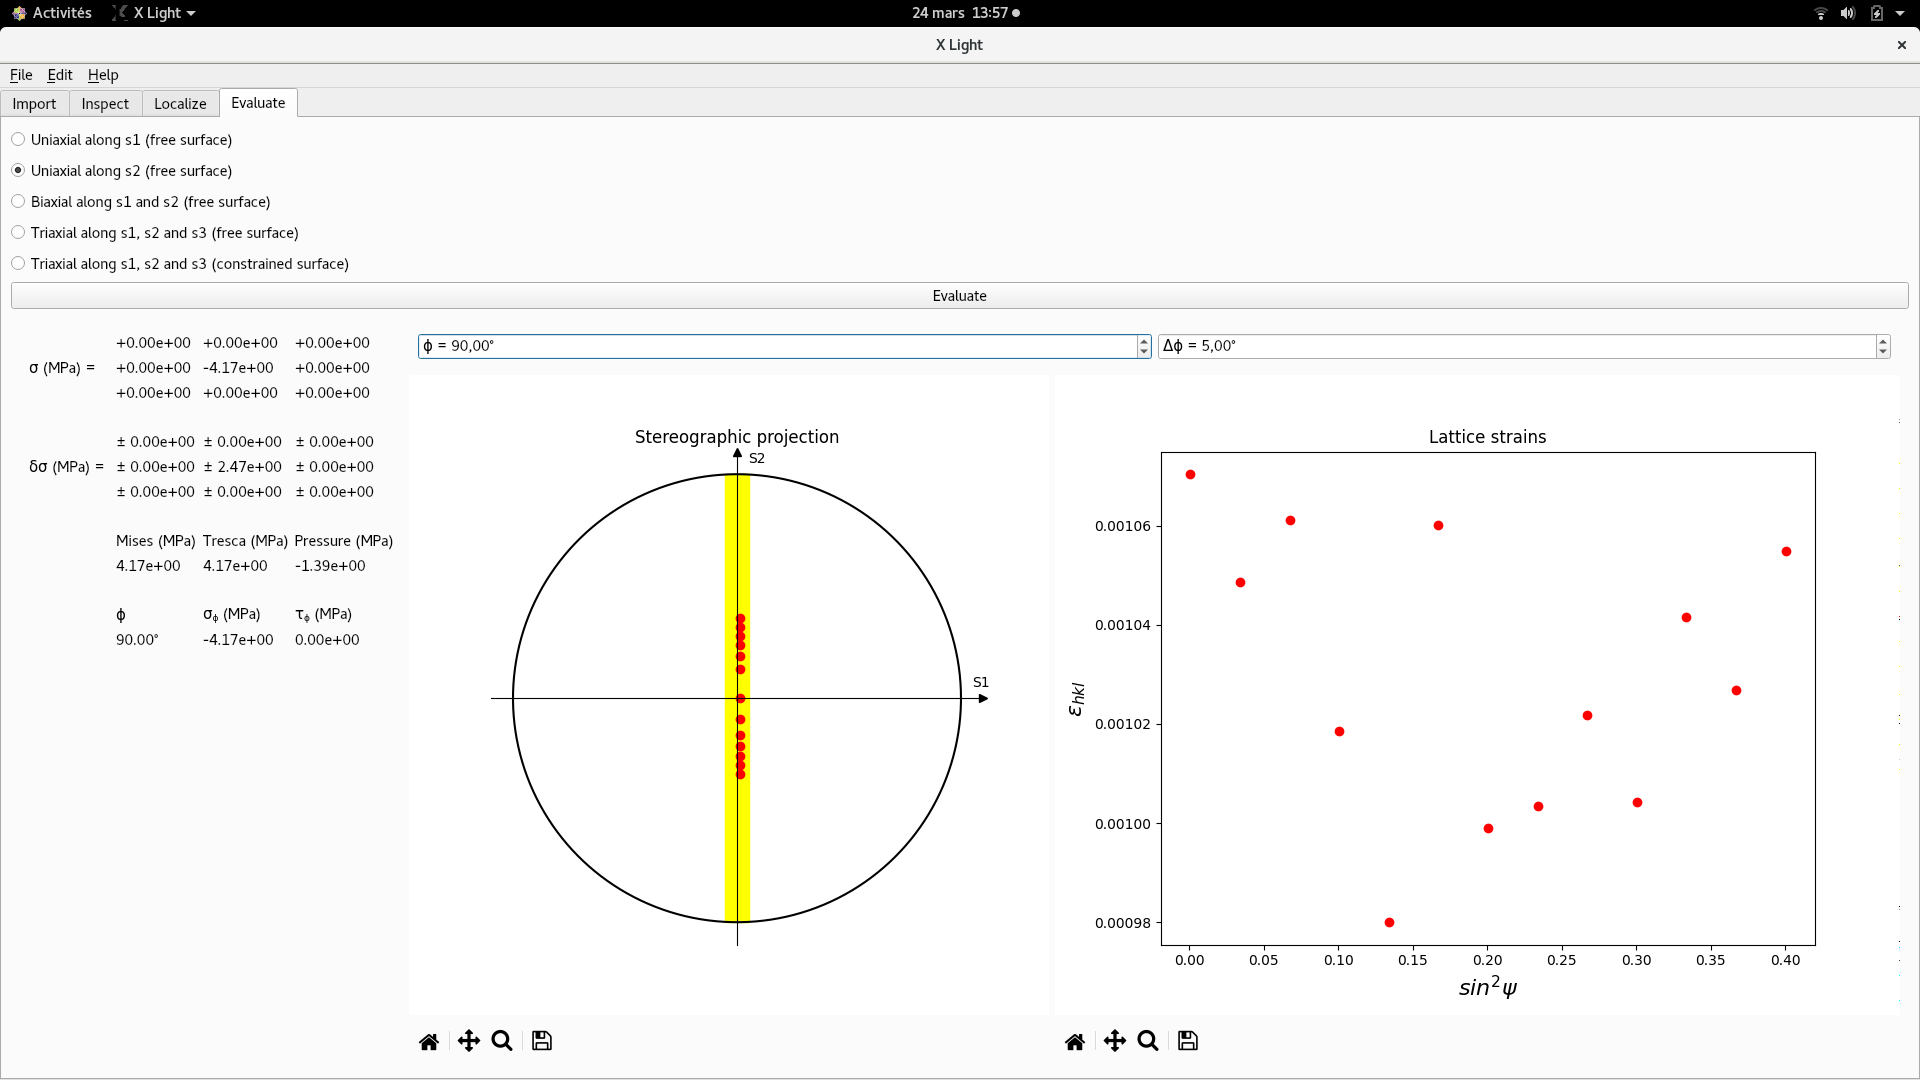
\includegraphics{figures/evaluate.png}}
\caption{Vue de l'onglet evaluation de l'interface d'X-Light.}
\label{fig_evaluate}
\end{figure}

Les directions de mesure correspondant aux différents pics de diffraction sont également représentés sur une figure de pôles, qui associe à chaque pic de diffraction la direction de mesure associée. Cette représentation permet notamment de distinguer les profils inactifs des profils actifs. Aussi, les déformations réticulaires $\varepsilon_{hkl}$ obtenues pour les différents pics de diffractions sont représentés sur un diagramme $\varepsilon_{hkl}-\sin^2 \Psi$. Sur ce diagramme sont regroupés les déformations associées à un angle $\Phi$, moyennant une certaine tolérance $\pm \Delta \Phi/2$. Ces deux valeurs peuvent être contrôlées \textit{via} l'interface.


\section{Base de données}

Pour la réalisation d'une analyse de contraintes, X-Light utilise un certains nombre de fichiers qui constitue la base de données du logiciel. L'utilisateur peut ajouter autant de fichiers que nécessaire. Il faut néanmoins qu'ils soient contenus dans les répertoires appropriés. Aussi, l'ajout de nouveaux fichiers dans la base de données n'est effectif qu'au prochain démarrage du logiciel.

\subsection{Fichier anode}

Les fichiers anode sont contenus dans le répertoire \textit{database/anodes}. Ils contiennent les valeurs des longueurs d'onde $K_{\alpha 1}$ et $K_{\alpha 2}$ ainsi que le rapport d'intensité $r$ entre ces longueurs d'onde. Le nom du fichier doit être du type \textit{Xy.txt} où \textit{Xy} désigne le symbole chimique de l'élément utilisé pour générer le rayonnement. A titre d'exemple, le contenu du fichier \textit{Mo.txt} est~:\\
\texttt{***Mo wavelength (Ka1, Ka2, R)} \\
\texttt{0.709300   0.713590  0.5}

\label{sec_fichieranode}

\subsection{Fichier détecteur}

Les fichiers détecteur sont contenus dans le répertoire \textit{database/detectors}. Ils fournissent l'ensemble des informations relatives à un détecteur bidimensionnel à savoir~:
\begin{itemize}
\item{le nombre de pixels selon les directions horizontale et verticale,}
\item{la taille de pixels selon les directions horizontale et verticale,}
\item{les coordonnées du centre du détecteur,}
\item{la distance entre le centre du détecteur et le centre goniométrique,}
\item{les paramètres du masque octahédral qui permet de définir la zone active du détecteur.}
\end{itemize}
Il est important de savoir que ces paramètres correspondent à des valeurs par défaut. Si des valeurs différentes sont trouvées lors de l'importation des données, ces nouvelles valeurs viennent remplacer les valeurs par défaut. A titre d'exemple, le descriptif d'un détecteur VANTEC V500 est donné par~:\\
\texttt{***DETECTOR: PXC-V500} \\
\texttt{***NUMBER OF PIXELS (nx, ny)} \\
\texttt{2048     2048} \\
\texttt{***PIXEL SIZE (deltax, deltay)} \\
\texttt{0.068    0.068} \\
\texttt{***DETECTOR CENTER (xc, yc)} \\
\texttt{1008.661      1011.721} \\
\texttt{***DISTANCE TO DETECTOR (d)} \\
\texttt{222.1785} \\
\texttt{***OCTMASK (MinX, MinX+Y, MinY, MaxX-Y, MaxX, MaxX+Y, MaxY, MaxY-X)} \\
\texttt{36  627  14  1416  2007  3458   2028  1415 } \\

\label{sec_fichierdetecteur}

\subsection{Fichier matériau}

Les fichiers matériaux sont stockés au sein du répertoire \textit{database/materials}. Chaque fichier est associé à un matériau particulier. Il contient les informations relatives à la nature du système réticulaire (\textit{CUBIC}, \textit{HEXAG}, \textit{TRIGO}, \textit{TETRA}, \textit{ORTHO}, \textit{MONOC} et \textit{TRICL}) ainsi que les paramètres de maille associés ($a$, $b$, $c$, $\alpha$, $\beta$ et $\gamma$). Aussi, les constantes d'élasticité sont données pour chaque famille de plans réticulaires $\{ hkl \}$ au travers du module de Young et du coefficient de Poisson. A titre d'exemple, le fichier matériau du nickel est présenté ci-après~:\\
\texttt{***Nickel XRD input file} \\
\texttt{*CRYSTAL SYSTEM} \\
\texttt{CUBIC} \\
\texttt{*LATTICE PARAMETERS (a,b,c,alpha,beta and gamma)} \\
\texttt{3.5239   3.5239   3.5239   90.   90.   90.} \\
\texttt{*PLANES (hkl)} \\
\texttt{1  1  1     264000   0.26} \\
\texttt{0  0  2     168000   0.35} \\
\texttt{2  2  0     231000   0.29} \\
\texttt{3  1  1     203000   0.32} \\
\texttt{2  2  2     264000   0.26} \\
\texttt{0  0  4     168000   0.35} \\
\texttt{3  3  1     240000   0.28} \\
\texttt{4  2  0     203000   0.32} \\
\label{sec_fichiermateriau}

% 
% eij=(1+v)/E sij - v/E smm 1ij
% 
% e=eij ni nj = (1+v)/E spq  np nq - v/E spq 1pq ni ni 

%     X-Light is a software dedicated to the evaluation of residual stresses using X-ray diffraction. The
% present document gives practical information on the use of X-Light for data acquired with a 2D
% detector. The calibration of the data is performed using pyFAI module, an open-source python
% module available on the web.
% The evaluation of residual stresses using X-ray diffraction data acquired with a 2D detector requires
% the calibration of the frames. This step consists in assigning to each pixel of the frame angular values
% in the (2θ,γ) space, 2θ being the diffraction angle and γ the azimuth angle, corresponding to (ψ,φ)
% values. In the following document, the distinction is made between the calibrant measurement
% (hereafter named calibrant), and the specimen of interest.


% Fin du document
\end{document}
